\documentclass[a4paper, 12pt]{article}
\usepackage[utf8]{inputenc}
\usepackage[T1]{fontenc}
\usepackage[scale=.8]{geometry}
\usepackage[french]{babel}
\usepackage{graphicx}

\title{Tunnel IPv6 sur IPv4}

\author{M1 Informatique \\\\ SCHNEEBERGER Thibault, CHAPUT Jean}
\date{}

\begin{document}
    \maketitle
    \newpage
    \tableofcontents
    \newpage

    \section{Configuration réseau}
    
    $$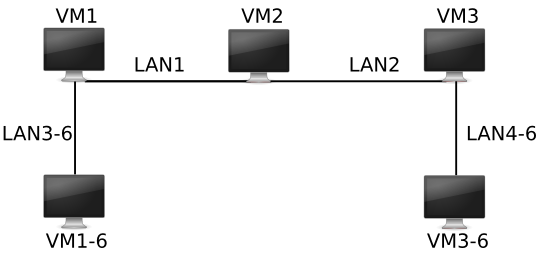
\includegraphics[scale=0.6]{images/topologie.png}$$ \\
    
    Pour démarrer, on s'intéresse à la réalisation du réseau de 5 machines
    proposé dans l'énoncé du sujet dont le schéma se trouve juste au dessus. 
    Pour cela, on reprend notre configuration du TP précédent en y apportant 
    quelques modifications. Premièrement, on supprime la configuration de la 
    deuxième interface dans les fichiers de configuration ansible sur les 
    machines \verb+VM1-6+ et \verb+VM3-6+ car ces machines n'en auront plus 
    la nécessité. (Cela n'est pas nécessaire pour le bon fonctionnement mais ça
    permet de faire un peu de propre). On supprime de plus les routes devenues 
    obsolètes permettant auparavant le passage par \verb+VM2-6+ pour la communication 
    en \verb+IPv6+.

    \section{Interface virtuelle}
    Une fois notre configuration terminée avec ansible, on s'intéresse 
    maintenant à la création et à la configuration d'une interface virtuelle
    \verb+TUN+ qui nous permettra d'effectuer la communication entre l'espace 
    noyau (d'où provient une trame échangée sur le réseau) vers l'espace 
    utilisateur (où se trouvera le code de notre tunnel).

    \subsection{Création de l'interface}
    Afin de créer l'interface virtuelle \verb+TUN+, on récupère le code fourni 
    contenu dans le fichier \verb+tunalloc.c+. Celui-ci contient la fonction 
    \verb+tun_alloc()+ et une fonction principale \verb+main()+. Lorsque l'on 
    regarde d'un peu plus près la fonction \verb+tun_alloc()+, on remarque que 
    lors de son appel elle retourne un entier. Il s'agit du descripteur de 
    fichier permettant la lecture ou bien l'écriture sur cette interface. \\

    On crée donc une bibliothèque \verb+iftun+, c'est-à-dire un fichier 
    d'en-tête \verb+iftun.h+ et un fichier source \verb+iftun.c+ afin d'y 
    ajouter la fonction \verb+tun_alloc()+. En plus de cela on crée un fichier 
    principal avec une fonction \verb+main()+ nous permettant d'effectuer les 
    tests de cette partie et les suivants.

    \subsection{Configuration de l'interface}
    Pour configurer l'interface \verb+TUN+, on a besoin de lui attribuer une 
    addresse \verb+IPv6+. Nous utiliseront l'adresse \verb+fc00:1234:ffff::1+ 
    avec le masque en \verb+/32+. On choisit un masque en \verb+/32+ car on 
    remarque qu'à la création de \verb+tun0+ une route est ajoutée vers 
    \verb+fc00:1234::/32+. Cela permettra le routage des paquets entrants en 
    direction de \verb+LAN4-6+ ou \verb+LAN3-6+ via l'interface \verb+tun0+ et
    donc le tunnel. Comme rappelé un peu plus haut il est aussi nécessaire de 
    modifier les configurations créées au TP précédent car dans notre cas 
    certaines routes ne sont plus valides. Par exemple pour \verb+VM1+ et 
    \verb+VM1-6+, dans le cas où ces machines voudraient communiquer avec 
    \verb+VM3-6+, elles ne pourront plus passer par \verb+VM2-6+. \\

    On crée donc un script \verb+configure_tun.sh+ qui contiendra les commandes
    de configuration de l'interface virtuelle. suivantes.
    \verb+ip address add fc00:1234:ffff::1/64 dev tun0+ pour lui ajouter 
    l'adresse \verb+IP+. Mais aussi la commande \verb+ip link set dev tun0 up+
    afin d'activer l'interface qui était pour le moment en état \verb+down+ 
    après sa création \\

    Afin de tester notre configuration et après avoir lancé notre programme de 
    test sur \verb+VM1+, on tente d'effectuer un \verb+ping -6+ de \verb+VM1-6+
    vers l'interface \verb+tun0+ sur \verb+VM1+. Celui-ci se déroule sans 
    problème et reçoit une réponse. Cependant, si l'on effectue une capture 
    wireshark sur \verb+VM1+, on se rend compte que les échanges ne passent pas 
    par \verb+tun0+. En effet, celle-ci ne capte aucune trame. Cela peut 
    s'expliquer car lorsque la trame envoyée par \verb+VM1-6+ arrive sur 
    \verb+VM1+ par son interface \verb+eth2+ (passerelle par défaut de 
    \verb+VM1-6+) elle est désencapsulée afin de regarder qui est le 
    destinataire pour pouvoir lui transmettre dans une nouvelle trame. Voyant
    que le destinataire est en réalité lui-même, le routeur \verb+VM1+ peut 
    traiter la demande et envoyer sa réponse. Cela se déroule dans l'espace 
    noyau. \\

    On effectue ensuite le test en faisant un \verb+ping -6+ depuis \verb+VM1+
    vers l'addresse \verb+IPv6+ suivante : \\ \verb+fc00:1234:ffff::10+. Cette 
    fois-ci le ping ne reçoit pas de réponse mais en effectuant une analyse de 
    paquets avec wireshark sur \verb+VM1+, on se rend compte que les paquets 
    sont transmis depuis l'interface \verb+eth2+ de \verb+VM1+ vers \verb+tun0+
    .Le ping ne reçoit ainsi pas de réponse car pour le moment les paquets 
    injectés dans \verb+tun0+ ne sont pas traités. Attention car pour cette 
    partie il faut bien penser à ajouter le drapeau de routage \verb+IPv6+ sur 
    \verb+VM1+ (et par symétrie sur \verb+VM3+) sinon la transmission entre 
    interfaces d'une même machine ne pourra pas s'effectuer. 

    \subsection{Récupération des paquets}
    Maintenant que l'on sait que les paquets sont redirigés sur l'interface
    virtuelle \verb+tun0+ dont nous disposons du descripteur de fichier, on 
    peut s'intéresser à la récupération des informations depuis \verb+tun0+. 
    On complète donc notre bibliothèque \verb+iftun+ avec une nouvelle fonction
    transfert qui permettra de transférer les données lues sur un descripteur 
    de fichier source vers un descripteur de fichier destination. \\

    On effectue donc le test de cette fonction avec comme descripteur de 
    fichier source celui retourné par la création de l'interface \verb+tun0+ et
    comme descripteur de fichier destination 1 (qui correspond à la 
    sortie standard). On effectue à nouveau les pings réalisés précédemment
    depuis \verb+VM1-6+. Au niveau du réseau rien ne change, Les captures sont 
    identiques. Cependant, on observe les paquets entrants sur \verb+tun0+ 
    s'afficher dans le terminal. Ceux-ci étant en binaire, on les rends plus 
    lisibles en filtrant l'affichage avec \verb+hexdump+ afin de rendre cela 
    plus lisible. \\

    Différentes options sont disponibles lorsque l'on crée l'interface 
    virtuelle. On peut utiliser les flags suivants: \verb+IFF_TUN+, 
    \verb+IFF_TAP+ et \verb+IFF_NO_PI+. \verb+IFF_TUN+ est celui que l'on 
    utilise car il permet de supprimer les en-têtes Ethernet afin de ne garder
    que le datagramme IP. \verb+IFF_NO_PI+ permet de retirer les 4 octets 
    concernant la version du protocole de couche IP. Le flag \verb+IFF_NO_PI+ 
    peut s'ajouter en plus du flag \verb+IFF_TUN+, les flags sont cumulables.

    \section{Un tunnel simple pour IPv6}

    Afin de faire communiquer \verb+VM1+ et \verb+VM3+ qui sont reliés par le 
    biais de \verb+VM2+ en \verb+IPv4+, on utilisera la connexion par socket à
    l'image d'un client et d'un serveur. Pour cela on crée une nouvelle 
    bibliothèque \verb+extremite+ qui contiendra les fonctions nécessaires à
    l'envoi et à la réception des datagrammes.

    \subsection{Redirection du traffic entrant}

    Afin de rediriger le traffic lu depuis \verb+tun0+ vers notre réseau 
    \verb+IPv4+, il nous faut créer une fonction \verb+ext_in()+ qui aura en 
    réalité un rôle de client et qui sera chargée d'ouvrir une connexion avec 
    l'autre extrémité du tunnel afin de lui envoyer tout ce qui est lu. Après 
    avoir ouvert une connexion distante sur sa socket, on peut simplement 
    effectuer un appel à notre fonction \verb+transfert()+ de la bibliothèque 
    \verb+iftun+. Celle-ci prend deux descripteurs de fichiers en paramètres, 
    le premier étant celui retourné par \verb+tun0+ et le deuxième la socket 
    en elle-même. \\

    En plus de la fonction \verb+ext_in()+, il nous faut aussi une fonction 
    \verb+ext_out()+ qui sera chargée du rôle de serveur et qui écoutera donc
    sur sa socket afin de rediriger dans un premier temps vers la sortie 
    standard (descripteur de fichier 1) afin de vérifier que tout fonctionne 
    correctement. La redirection est ici aussi effectuée à l'aide de la 
    fonction transfert de la bibliothèque \verb+iftun+. À terme le transfert ne
    s'effectuera plus vers la sortie standard mais bien sur le descripteur de 
    fichier de \verb+tun0+ afin de réinjecter notre datagramme \verb+IPv6+ dans
    le réseau. \\

    Lorque tout est mis en place, c'est à dire que le programme de test est
    lancé en mode client sur \verb+VM1+ et en mode serveur sur \verb+VM3+, on
    peut effectuer notre \verb+ping -6+ habituel depuis \verb+VM1-6+ vers 
    l'adresse \verb+fc00:1234:ffff::10+. Si l'on se place ensuite sur 
    \verb+VM3+, on voit l'ensemble des paquets arriver depuis le tunnel 
    s'afficher sur la sortie standard.

    \subsection{Redirection du traffic sortant}

    Maintenant qu'il est possible pour nous d'afficher le contenu du tunnel
    sur la sortie standard de \verb+VM3+, on veut pouvoir le rediriger vers son
    interface virtuelle \verb+tun0+. Cela aura pour but de réintégrer le 
    datagramme \verb+IPv6+ transporté par le tunnel sur \verb+IPv4+ dans le 
    réseau \verb+IPv6+. Pour cela il suffit de modifier la fonction 
    \verb+ext_out()+ de la bibliothèque \verb+extremite+ en effectuant un 
    transfert non plus vers 1 (sortie standard) mais vers le descripteur de
    fichier retourné par \verb+tun0+. \\

    De cette manière les datagrammes \verb+IPv6+ qui étaient transportés par un 
    datagramme \verb+IPv4+ dans le tunnel sont réintégrés dans un réseau 
    \verb+IPv6+ à la sortie de celui-ci. Cela permet à la machine \verb+VM3-6+ 
    de recevoir le ping provenant de \verb+VM1-6+. Pour vérifier le bon
    fonctionnement du tunnel, on peut prendre un datagramme \verb+IPv6+ avec
    comme adresse de destination la machine \verb+VM3-6+ et l'envoyer sur la
    socket d'écoute de la sortie du tunnel sur \verb+VM3+. On réalise cela à 
    l'aide de la commande \verb+nc 172.16.2.163 123 < datagramme-v6.bin+. On 
    se place sur VM3 et on observe le paquet entrant être redirigé vers 
    \verb+tun0+ puis arriver sur \verb+VM3-6+.

    \subsection{Intégration finale du tunnel}

    Maintenant que notre datagramme \verb+IPv6+ arrive à rejoindre notre second 
    réseau \verb+IPv6+, on cherche à faire fonctionner notre tunnel dans les 
    sens. Pour cela, il nous faut lancer les fonctions \verb+ext_in()+ et 
    \verb+ext_out()+ à chaque extrémité du tunnel. Afin que cela soit possible
    on décide de passer l'adresse \verb+IPv4+ de la sortie du tunnel en 
    paramètres de la fonction \verb+ext_in()+. Avec une modification de notre 
    fonction principale \verb+main()+, on lui permet de lancer le tunnel soit 
    sur \verb+VM1+ soit sur \verb+VM2+. \\

    Pour lancer à la fois la fonction \verb+ext_in()+ et la fonction 
    \verb+ext_out()+, on utilisera la librairie C \verb+pthreads+ qui permet 
    de lancer des threads d'exécution assez simplement au lieu d'utiliser les
    processus système avec des appels à \verb+fork()+. Pour pouvoir lancer ces
    threads depuis le main, on aura besoin d'une bibliothèque supplémentaire 
    que l'on nommera \verb+executeur+. Cette bibliothèque contient deux 
    pointeurs de fonctions qui font appel à \verb+ext_in()+ et \verb+ext_out()+.
    On crée aussi une structure de donnée permettant de passer les arguments
    nécessaires au lancement du tunnel à nos fonctions. \\

    Après avoir lancé le tunnel sur \verb+VM1+ et sur \verb+VM2+, on effectue 
    des pings entre \verb+VM1-6+ et \verb+VM3-6+. Pour vérifier que tout est
    bon on effectue une capture wireshark du traffic circulant sur \verb+VM2+
    en \verb+IPv4+. On effectue une seconde capture  sur \verb+VM3+ en 
    \verb+IPv6+. D'après l'analyse de ces captures situées dans le répertoire 
    \verb+docs+, tout est fonctionnel.

    \subsection{Mise en place du tunnel entre VM1 et VM3: Schémas}

    $$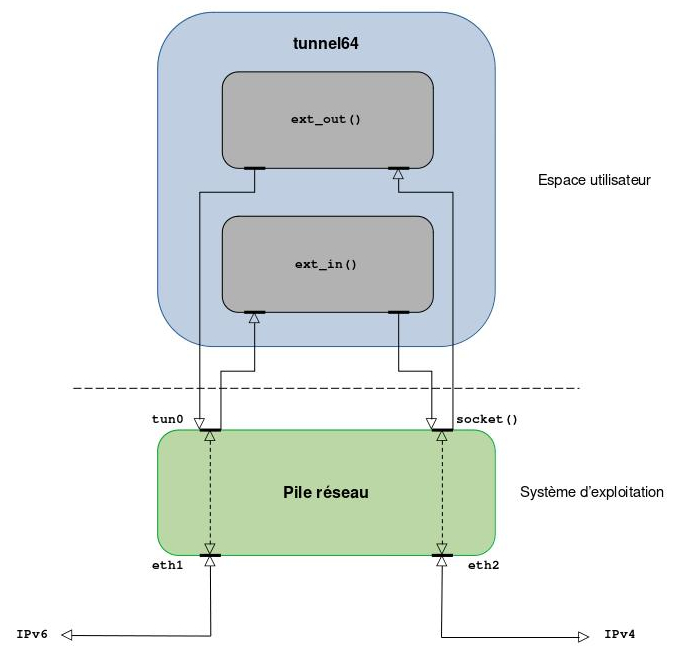
\includegraphics[scale=0.6]{images/schema_reseau.jpg}$$ \\

    Voici le schéma plus détaillé du fonctionnement du tunnel. Lorsqu'un 
    datagramme \verb+IPv6+ est à destination de l'autre extrémité du tunnel,
    il est lu sur l'interface virtuelle \verb+TUN+ (\verb+tun0+) et encapsulé 
    dans un datagramme \verb+IPv4+ en étant écrit sur la socket ouverte par la 
    fonction \verb+ext_in()+. Il est ensuite acheminé jusqu'à sa destination 
    (c'est-à-dire \verb+VM3+ dans notre cas) en empruntant le réseau \verb+IPv4+
    (\verb+LAN1+ et \verb+LAN2+ ici). A son arrivée à la sortie du tunnel, le 
    datagramme \verb+IPv6+ est désencapsulé du datagramme \verb+IPv4+ puis écrit 
    dans l'interface virtuelle \verb+TUN+ (\verb+tun0+) afin de rejoindre sa 
    destination en \verb+IPv6+.

    \subsection{Mise en place du tunnel entre VM1 et VM3: Système}

    Pour n'avoir qu'un simple exécutable permettant de démarrer le tunnel, on 
    s'intéresse à la lecture des paramètres de celui-ci depuis un fichier de 
    configuration \verb+tunnel64.conf+. On crée alors une bibliothèque de
    fonctions \verb+config+ dont le rôle est de récupérer les paramètres de 
    configuration dans le fichier afin de pouvoir les faire passer en argument
    de nos appels à \verb+ext_in()+ et \verb+ext_out()+. Une fois cela fait, 
    on peut essayer de démarrer le tunnel sur \verb+VM1+ et \verb+VM3+ avec la 
    commande \verb+./bin/tunnel64+ depuis le répertoire \verb+/mnt/partage/tunnel64+.
    Le tunnel se lance correctementet les pings entre \verb+VM1-6+ et \verb+VM3-6+ 
    sont fonctionnels.

    \section{Validation fonctionnelle}

    \subsection{Configuration}

    Sur chaque machine de notre réseau (\verb+VM1+, \verb+VM2+, \verb+VM2+, 
    \verb+VM1-6+ et \verb+VM3-6+) on récupère les paramètres réseaux 
    significatifs avec les commandes \verb+ip a+ et \verb+ip r+. L'ensemble 
    des résultats est cohérent avec ce que nous attendions. Si besoin est de
    les consulter, l'ensemble des fichiers texte contenant les résultats des 
    commandes se trouvent dans le répertoire \verb+docs/configs+. Les résultats 
    sont aussi disponibles en simples captures d'écran dans le répertoire 
    \verb+docs/images/configs+.

    \subsection{Couche 3}

    On se place sur \verb+VM1-6+ et on effectue un ping vers \verb+fc00:1234:4::36+.
    Celui-ci se termine sans erreur et nous donne les captures d'écran situées dans 
    le répertoire \verb+docs/images+. On effectue en plus deux captures à l'aide de 
    wireshark. Une en \verb+IPv4+ sur \verb+VM2+ et une en \verb+IPv6+ sur \verb+VM3+.
    Ces captures sont aussi disponibles dans le répertoire \verb+docs+. On y voit 
    notre datagramme \verb+IPv6+ envoyé par \verb+VM1-6+ circuler en données d'un 
    datagramme \verb+IPv4+ sur \verb+VM2+ puis on le retrouve sur le réseau 
    \verb+IPv6+ de \verb+VM3+ lorsqu'il est réintroduit sur \verb+tun0+.

    \subsection{Couche 4}

    Pour tester un peu plus en profondeur le fonctionnement du tunnel, on essaye
    de se connecter au service \verb+echo+ de \verb+VM3-6+ depuis \verb+VM1-6+.
    Pour cela on utilise la commande telnet suivante : 
    \verb+telnet fc00:1234:4::36 echo+. La connexion se déroule sans problème 
    et le service \verb+echo+ fonctionne correctement.

    \subsection{Couche 4 : bande passante}

    On s'intéresse maintenant à la performance de notre tunnel. Pour cela, nous 
    allons utiliser l'utilitaire \verb+iperf3+. On commence par le lancer en
    mode serveur sur \verb+VM3-6+ puis on essaye avec différentes tailles de 
    tampon depuis \verb+VM1-6+.

    \section{Améliorations}

    \subsection{Configuration via ansible}

    Puisque notre tunnel peut-être lancé simplement depuis le terminal, il 
    semble tout à fait possible de le lancer avec \verb+ansible+. Cependant pour
    pouvoir faire cela, il nous faut pouvoir lancer le tunnel en tâche de fond 
    afin que celui-ci ne soit pas interrompu lors de la fin de la configuration
    et à la fermeture du shell. Sur un système \verb+GNU/Linux+, on peut 
    utiliser la commande \verb+nohup+ qui permet de faire cela. \\

    Lorsque l'on utilise cette commande dans \verb+ansible+, on est confronté à 
    des erreurs qui sont générées par la sortie standard et la sortie d'erreur.
    Pour les éviter on redirige la sortie d'erreur vers la sortie standard et 
    la sortie standard vers \verb+/dev/null+. \\

    Une fois tout cela fait, lorsqu'on lance la configuration de \verb+VM1+
    et \verb+VM3+ via ansible avec la commande \verb+ansible-playbook /vagrant/config.yml+, 
    le tunnel se lance. On peut le vérifier en faisant \verb+ip a+ sur l'une
    des deux extrémités du tunnel, \verb+tun0+ est encore affichée, ce qui 
    signifie que le tunnel tourne encore. Pour vérifier qu'il fonctionne 
    correctement on effectue à nouveau un ping depuis \verb+VM1-6+ vers 
    \verb+VM3-6+ avec succès.

\end{document}

/